\chapter{Aromatisitas dan Substitusi Aromatik Elektrofilik}\label{ch:b2:aromatic-substitution}

Air brom kehilangan warnanya dalam beberapa detik jika dikocok dengan
alkena, dan sama sekali tidak jika dikocok dengan benzena. Namun benzena
memang bereaksi dengan brom begitu sedikit besi(III) bromida ditambahkan ---
dan produknya, bromobenzena, masih mempunyai cincin \omterm{def:b2:huckel:aromatic}{aromatik} beranggota
enamnya: satu hidrogen telah digantikan, tidak ada yang diadisikan.
Cincin \omterm{def:b2:huckel:aromatic}{aromatik} mengalami substitusi alih-alih adisi, karena adisi akan
membuang stabilisasi yang dihitung pada \cref{ch:b2:huckel}. Mekanisme yang
sama menitrasi, menyulfonasi, mengalkilasi, dan mengasilasi cincin benzena,
dan gugus-gugus yang sudah ada pada cincin menentukan, dengan keteraturan
yang mengejutkan, ke mana gugus berikutnya masuk.

\begin{recall}
\Cref{ch:b2:huckel}: aromatisitas dan \omterm{def:b2:huckel:delocalisation}{energi delokalisasi} benzena. Jilid
Tahun 1: adisi elektrofilik pada alkena, efek induktif dan mesomerik, gugus
donor dan akseptor, karbokation dan penataan ulangnya, postulat Hammond,
asam Lewis, profil energi.
\end{recall}

\begin{omfigure}
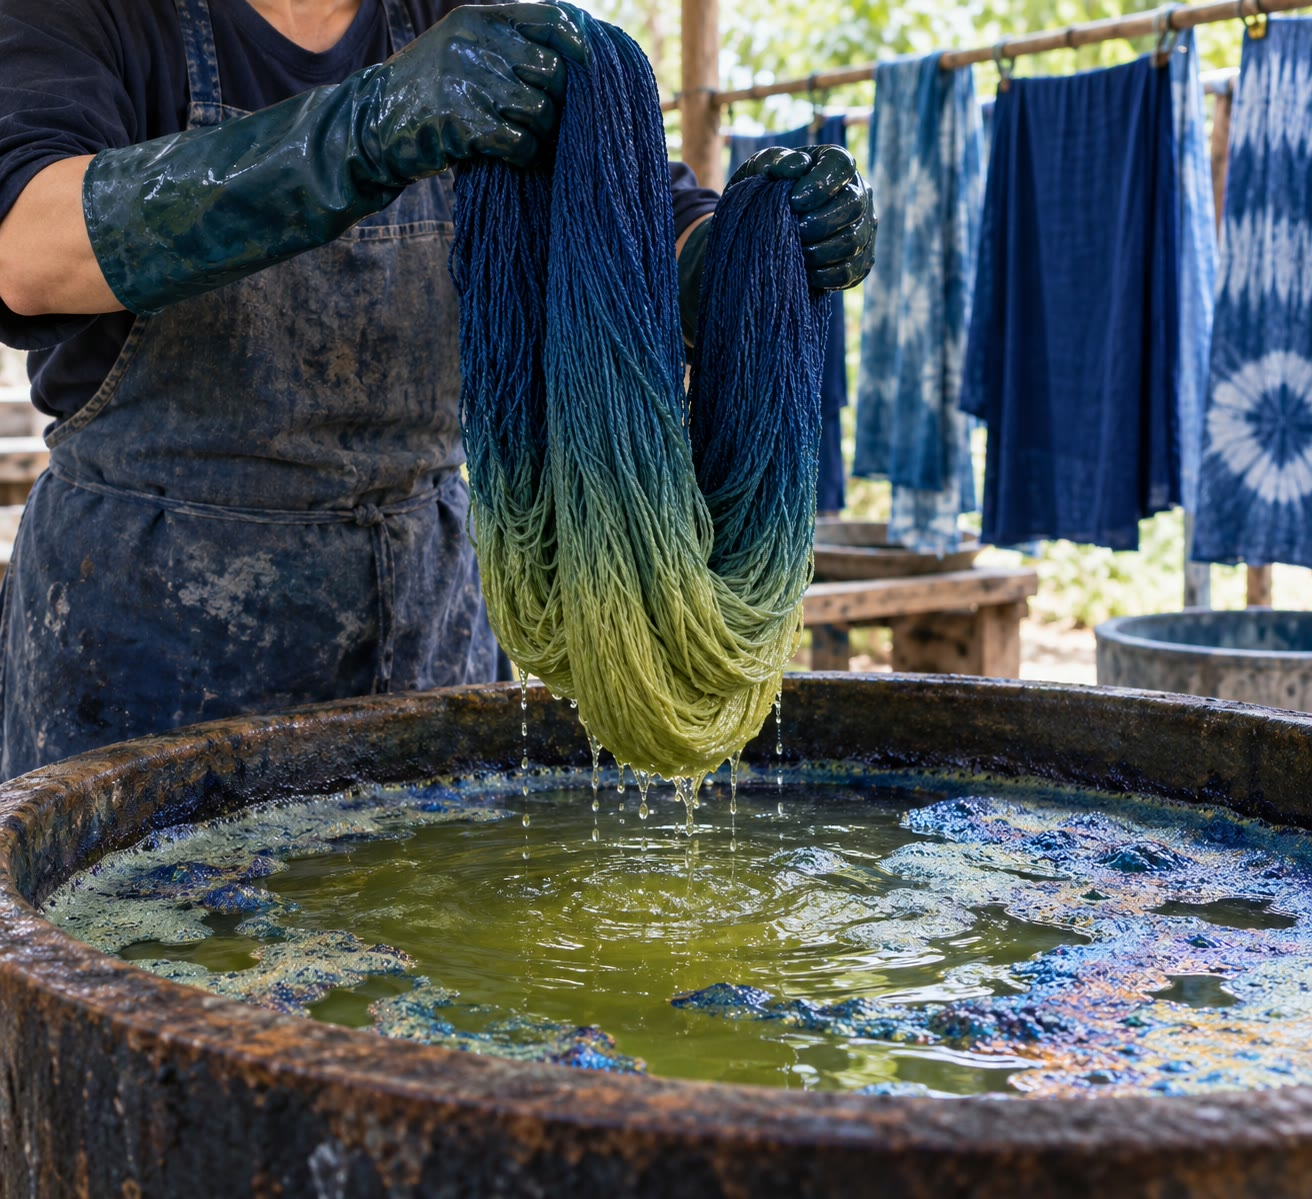
\includegraphics[width=0.55\linewidth]{images/book3/ai/b2-22-indigo-vat-2.jpg}

{\small Mencelup benang dalam bejana indigo (ilustrasi). Benang meninggalkan
bejana berwarna kuning kehijauan, terendam bentuk tereduksi zat warna yang
larut, dan menjadi biru di udara ketika oksigen mengubahnya kembali menjadi
indigo yang tidak larut. Indigo, seperti kebanyakan zat warna, dibangun di
atas cincin-cincin \omterm{def:b2:huckel:aromatic}{aromatik}; industri zat warna abad kesembilan belas tumbuh
dari reaksi-reaksi substitusi dalam bab ini yang diterapkan pada benzena dari
ter batu bara.}
\end{omfigure}

\section{Substitusi, bukan adisi}

\begin{definition}[Arena]\label{def:b2:aromatic-substitution:arene}
Yang disebut \emph{arena}\index{arena} adalah hidrokarbon yang mengandung
sekurang-kurangnya satu cincin \omterm{def:b2:huckel:aromatic}{aromatik}, seperti benzena, toluena
(metilbenzena), atau naftalena; gugus aril (\ce{Ar}) adalah arena yang
kehilangan satu hidrogen.
\end{definition}

\begin{proposition}[Mengapa benzena tidak mengalami adisi]\label{prop:b2:aromatic-substitution:no-addition}
Adisi pada benzena akan mengubah cincin \omterm{def:b2:huckel:aromatic}{aromatik} menjadi sikloheksadiena
yang tidak \omterm{def:b2:huckel:aromatic}{aromatik} dan kehilangan sebagian besar dari \qty{150}{kJ/mol}
stabilisasi \omterm{def:b2:huckel:aromatic}{aromatik}; substitusi mempertahankannya.
\end{proposition}

\begin{proof}[Argumen]
Pada \cref{ch:b2:huckel}, hidrogenasi benzena menjadi sikloheksa-1,3-diena
ternyata \omterm{def:b2:reaction-enthalpy:exothermic}{endoterm} (\qty{+22}{kJ/mol}, dari \qty{-206.0}{} dan
\qty{-227.7}{kJ/mol}), sedangkan hidrogenasi ikatan rangkap biasa melepaskan
\qty{119}{kJ/mol}: adisi pertama adalah tahap yang mahal.
Setelah tahap elektrofilik pertama, kation yang terbentuk dapat mengadisi
nukleofil, yang menyisakan \omterm{def:b2:frontier-orbitals:diels-alder}{diena} yang tidak \omterm{def:b2:huckel:aromatic}{aromatik}, atau melepaskan
proton, yang memulihkan cincin \omterm{def:b2:huckel:aromatic}{aromatik}. Jalur kedua jauh lebih
menguntungkan.
% ledger: dfh:C6H6_g, dfh:C6H8_g, dfh:C6H10_g, dfh:C6H12_g
\end{proof}

\section{Mekanisme}

\begin{definition}[Substitusi aromatik elektrofilik]\label{def:b2:aromatic-substitution:seAr}
Yang disebut \emph{substitusi aromatik elektrofilik}\index{substitusi aromatik elektrofilik}
menggantikan sebuah hidrogen cincin \omterm{def:b2:huckel:aromatic}{aromatik} dengan elektrofil \ce{E+}.
Elektrofil itu mula-mula berikatan dengan satu karbon cincin, sehingga
terbentuk kation yang karbon itu tetrahedral dan muatan positifnya tersebar
pada kelima karbon lainnya: \emph{zat antara Wheland}\index{zat antara Wheland}
(ion arenium). Sebuah basa lalu mengambil proton dari karbon yang tetrahedral itu.
\end{definition}

\begin{proposition}[Dua tahap]\label{prop:b2:aromatic-substitution:mechanism}
Tahap pertama, yang merusak aromatisitas, adalah tahap yang lambat;
lepasnya proton, yang memulihkannya, berlangsung cepat.
\end{proposition}

\begin{proof}[Argumen]
\omterm{def:b2:aromatic-substitution:seAr}{Zat antara Wheland} adalah karbokation yang distabilkan oleh delokalisasi
pada tiga karbon tetapi tidak \omterm{def:b2:huckel:aromatic}{aromatik}: zat antara itu terletak jauh di atas
pereaksi, dan menurut postulat Hammond keadaan transisi yang menuju ke sana
mirip dengannya dalam struktur dan energi. Tahap kedua turun menuju produk
\omterm{def:b2:huckel:aromatic}{aromatik}: penghalangnya rendah.
\end{proof}

\begin{omfigure}
\begin{tikzpicture}
\begin{axis}[width=0.55\linewidth, height=5.4cm, xmin=-0.2, xmax=4.2, ymin=-5.5, ymax=11.5,
  axis x line=bottom, axis y line=left, xtick=\empty, ytick=\empty,
  xlabel={koordinat reaksi}, ylabel={energi}, label style={font=\small}, clip=false]
\addplot[omDef, thick] table[x=x, y=sub] {figdata/out/bachelor-2-aromatic-profile.dat};
\addplot[omThm, thick, dashed, restrict x to domain=2:4] table[x=x, y=add] {figdata/out/bachelor-2-aromatic-profile.dat};
\node[font=\scriptsize, anchor=north west] at (axis cs:0.0,-0.6) {\ce{ArH + E+}};
\node[font=\scriptsize, anchor=north] at (axis cs:2,5.7) {Wheland};
\node[font=\scriptsize, anchor=west, omDef] at (axis cs:4.05,-4.0) {\ce{ArE + H+}};
\node[font=\scriptsize, anchor=west, omThm] at (axis cs:4.05,2.0) {produk adisi};
\node[font=\scriptsize, anchor=south] at (axis cs:1,10.1) {lambat};
\end{axis}
\end{tikzpicture}

{\small Profil energi \omterm{def:b2:aromatic-substitution:seAr}{substitusi aromatik elektrofilik}, skematis (sebuah
model). Tahap pertama, yang membentuk \omterm{def:b2:aromatic-substitution:seAr}{zat antara Wheland}, mempunyai
penghalang tertinggi. Lepasnya proton (garis penuh) memulihkan cincin
\omterm{def:b2:huckel:aromatic}{aromatik}; adisi nukleofil (putus-putus) akan menyisakan produk di atas
pereaksi.}
\end{omfigure}

\begin{omfigure}
\setchemfig{atom sep=2em}
\schemestart
\chemfig{HO-\chemabove{N}{\scriptstyle +}(=[1]O)-[7]\chemabove{O}{\scriptstyle -}} \+ \chemfig{H_2SO_4}
\arrow{<=>}
\chemfig{O=N^{+}=O} \+ \chemfig{HSO_4^{-}} \+ \chemfig{H_2O}
\schemestop

\medskip
\begin{tikzpicture}[font=\small, >={Stealth}]
\tikzset{pics/whel/.style n args={4}{code={
    \foreach \k in {0,...,5} \draw[thick] ({90+60*\k}:0.7) -- ({150+60*\k}:0.7);
    \foreach \k in {#1} \draw[thick] ($({90+60*\k}:0.56)!0.18!({150+60*\k}:0.56)$) -- ($({90+60*\k}:0.56)!0.82!({150+60*\k}:0.56)$);
    \ifnum#2>-1 \node[font=\scriptsize] at ({90+60*#2}:0.36) {$+$};\fi
    \draw[thick] (270:0.7) -- ++(-125:0.42) node[anchor=north east, inner sep=1pt, font=\scriptsize] {H};
    \draw[thick] (270:0.7) -- ++(-55:0.42) node[anchor=north west, inner sep=1pt, font=\scriptsize] {#4};
    \if\relax\detokenize{#3}\relax\else
      \draw[thick] (90:0.7) -- (90:1.1) node[anchor=south, inner sep=1pt, font=\scriptsize] {#3};\fi
  }}}
  \foreach \k in {0,...,5} \draw[thick] ({90+60*\k}:0.7) -- ({150+60*\k}:0.7);
  \foreach \k in {0,2,4} \draw[thick] ($({90+60*\k}:0.56)!0.18!({150+60*\k}:0.56)$) -- ($({90+60*\k}:0.56)!0.82!({150+60*\k}:0.56)$);
  \node at (1.3,0) {$+$};
  \node at (2.0,0) {\ce{NO2+}};
  \draw[->, thick] (2.6,0) -- (3.8,0) node[midway, above, font=\scriptsize] {lambat};
  \pic at (4.7,0.1) {whel={1,4}{0}{}{\ce{NO2}}};
  \draw[->, thick] (5.6,0) -- (6.8,0) node[midway, above, font=\scriptsize] {cepat} node[midway, below, font=\scriptsize] {$-$\ce{H+}};
  \begin{scope}[xshift=7.7cm]
    \foreach \k in {0,...,5} \draw[thick] ({90+60*\k}:0.7) -- ({150+60*\k}:0.7);
    \foreach \k in {0,2,4} \draw[thick] ($({90+60*\k}:0.56)!0.18!({150+60*\k}:0.56)$) -- ($({90+60*\k}:0.56)!0.82!({150+60*\k}:0.56)$);
    \draw[thick] (270:0.7) -- (270:1.1) node[anchor=north, font=\scriptsize] {\ce{NO2}};
  \end{scope}
\end{tikzpicture}
\par\vspace{6pt}

{\small Nitrasi benzena. Asam sulfat memprotonasi asam nitrat, yang lalu
melepaskan air: ion nitronium \ce{NO2+} adalah elektrofilnya. Ion itu
berikatan dengan satu karbon (lambat) dan menghasilkan \omterm{def:b2:aromatic-substitution:seAr}{zat antara Wheland},
yang muatan positifnya tersebar pada cincin; lepasnya proton (cepat)
menghasilkan nitrobenzena.}
\end{omfigure}

\section{Reaksi-reaksinya}

\paragraph{Halogenasi.} Brom atau klor saja merupakan elektrofil yang
terlalu lemah; asam Lewis (\ce{FeBr3}, \ce{AlCl3}) memolarkan halogen dengan
mengikat salah satu atomnya, dan atom brom yang di luar menyerang cincin.

\paragraph{Nitrasi.} Campuran asam nitrat dan asam sulfat pekat (di atas)
menghasilkan ion nitronium.

\paragraph{Sulfonasi.} Asam sulfat berasap (\ce{SO3} dalam \ce{H2SO4})
menghasilkan asam benzenasulfonat. Reaksi ini reversibel: memanaskan asam
sulfonat dalam asam berair encer melepaskan kembali gugus \ce{SO3H}, sehingga
gugus itu berguna sebagai gugus pemblokir sementara.

\begin{definition}[Reaksi Friedel--Crafts]\label{def:b2:aromatic-substitution:friedel-crafts}
Yang disebut \emph{alkilasi Friedel--Crafts}\index{alkilasi Friedel--Crafts}
memasang gugus alkil pada cincin \omterm{def:b2:huckel:aromatic}{aromatik} dari haloalkana dan asam Lewis
(\ce{AlCl3}). Yang disebut \emph{asilasi
Friedel--Crafts}\index{asilasi Friedel--Crafts} memasang gugus asil
\ce{RCO} dari asil klorida dan \ce{AlCl3}, melalui \emph{ion asilium}\index{ion asilium}
\ce{R-C#O+}, dan menghasilkan aril keton.
\end{definition}

\begin{proposition}[Batas reaksi Friedel--Crafts]\label{prop:b2:aromatic-substitution:friedel-crafts-limits}
\omterm{def:b2:aromatic-substitution:friedel-crafts}{Alkilasi Friedel--Crafts} terganggu oleh penataan ulang karbokation dan oleh
polialkilasi; asilasi berhenti setelah satu substitusi, tidak mengalami
penataan ulang, dan memerlukan sekurang-kurangnya satu ekuivalen
\ce{AlCl3}. Tidak satu pun bekerja pada cincin yang membawa \omterm{def:b2:aromatic-substitution:directing}{gugus pendeaktif}
kuat.
\end{proposition}

\begin{proof}[Argumen]
Elektrofil pengalkil adalah karbokation (atau kompleks terpolarisasi yang
berperilaku seperti karbokation), yang mengalami penataan ulang menjadi
karbokation yang lebih stabil melalui pergeseran hidrida atau alkil:
1-kloropropana terutama menghasilkan isopropilbenzena. Gugus alkil
mengaktifkan cincin (subbab berikutnya), sehingga produknya bereaksi lebih
cepat daripada benzena dan teralkilasi lagi. \omterm{def:b2:aromatic-substitution:friedel-crafts}{Ion asilium} distabilkan oleh
resonansi (\ce{R-C+=O} $\leftrightarrow$ \ce{R-C#O+}) dan tidak mengalami
penataan ulang; gugus asil mendeaktifkan cincin, sehingga produknya tidak
bereaksi lebih lanjut; dan keton yang terbentuk mengikat \ce{AlCl3} melalui
oksigennya, sehingga mengeluarkan katalis dari reaksi: satu ekuivalen
terpakai. Cincin yang sangat terdeaktivasi merupakan nukleofil yang terlalu
buruk untuk elektrofil-elektrofil lemah ini.
\end{proof}

\section{Efek substituen}

\begin{definition}[Gugus pengarah]\label{def:b2:aromatic-substitution:directing}
Sebuah substituen pada cincin benzena adalah \emph{gugus pengaktif}\index{gugus pengaktif}
jika cincinnya bereaksi lebih cepat daripada benzena, dan \emph{gugus
pendeaktif}\index{gugus pendeaktif} jika bereaksi lebih lambat. Substituen
itu adalah \emph{pengarah orto/para}\index{pengarah orto/para} jika gugus
yang baru terutama masuk pada posisi-posisi di sebelahnya dan di
seberangnya, dan \emph{pengarah meta}\index{pengarah meta} jika gugus itu
terutama masuk pada posisi-posisi yang berselang satu.
\end{definition}

\begin{proposition}[Donor dan akseptor]\label{prop:b2:aromatic-substitution:directing}
Gugus-gugus yang menyumbangkan elektron kepada cincin melalui efek mesomerik
(\ce{-OH}, \ce{-OCH3}, \ce{-NH2},
\ce{-NHCOCH3}) atau melalui efek induktif dan \omterm{def:b2:fragment-orbitals:hyperconjugation}{hiperkonjugasi} (alkil)
mengaktifkan cincin dan mengarahkan ke orto/para. Gugus-gugus yang menarik
elektron melalui efek mesomerik (\ce{-NO2}, \ce{-CN}, \ce{-COR},
\ce{-COOH}, \ce{-SO3H}) mendeaktifkannya dan mengarahkan ke meta.
\end{proposition}

\begin{proof}
Bandingkan zat-zat antara Wheland. Untuk serangan orto atau para terhadap
substituen G, salah satu dari ketiga struktur resonansi menempatkan muatan
positif pada karbon yang membawa G; untuk serangan meta, tidak ada yang
demikian. Donor G (pasangan elektron bebas pada O atau N) menstabilkan
muatan positif pada karbon tempat ia terikat, dengan menambahkan struktur
resonansi keempat yang setiap atomnya beroktet: zat antara orto dan para
turun, dan menurut postulat Hammond demikian pula keadaan-keadaan transisi
yang menuju ke sana. Akseptor G mendestabilkan muatan positif pada
karbonnya: zat antara orto dan para naik, dan serangan meta, yang
menghindari struktur itu, menjadi yang paling sedikit dirugikan, walaupun
lebih lambat daripada pada benzena.
\end{proof}

\begin{omfigure}
\begin{tikzpicture}[font=\small]
\tikzset{pics/whel/.style n args={4}{code={
    \foreach \k in {0,...,5} \draw[thick] ({90+60*\k}:0.7) -- ({150+60*\k}:0.7);
    \foreach \k in {#1} \draw[thick] ($({90+60*\k}:0.56)!0.18!({150+60*\k}:0.56)$) -- ($({90+60*\k}:0.56)!0.82!({150+60*\k}:0.56)$);
    \ifnum#2>-1 \node[font=\scriptsize] at ({90+60*#2}:0.36) {$+$};\fi
    \draw[thick] (270:0.7) -- ++(-125:0.42) node[anchor=north east, inner sep=1pt, font=\scriptsize] {H};
    \draw[thick] (270:0.7) -- ++(-55:0.42) node[anchor=north west, inner sep=1pt, font=\scriptsize] {#4};
    \if\relax\detokenize{#3}\relax\else
      \draw[thick] (90:0.7) -- (90:1.1) node[anchor=south, inner sep=1pt, font=\scriptsize] {#3};\fi
  }}}
  \node[anchor=east] at (-1.0,0) {metoksi, serangan para:};
  \pic at (0,0) {whel={1,4}{0}{\ce{OCH3}}{E}};
  \node at (1.25,0.1) {$\leftrightarrow$};
  \begin{scope}[xshift=2.5cm]
    \foreach \k in {0,...,5} \draw[thick] ({90+60*\k}:0.7) -- ({150+60*\k}:0.7);
    \foreach \k in {1,4} \draw[thick] ($({90+60*\k}:0.56)!0.18!({150+60*\k}:0.56)$) -- ($({90+60*\k}:0.56)!0.82!({150+60*\k}:0.56)$);
    \draw[thick] (-0.06,0.7) -- (-0.06,1.1); \draw[thick] (0.06,0.7) -- (0.06,1.1);
    \node[anchor=south, inner sep=1pt, font=\scriptsize] at (0,1.1) {$\overset{+}{\mathrm O}\mathrm{CH_3}$};
    \draw[thick] (270:0.7) -- ++(-125:0.42) node[anchor=north east, inner sep=1pt, font=\scriptsize] {H};
    \draw[thick] (270:0.7) -- ++(-55:0.42) node[anchor=north west, inner sep=1pt, font=\scriptsize] {E};
  \end{scope}
  \node[anchor=west, font=\scriptsize] at (3.4,0) {struktur tambahan, setiap atom beroktet};
  \begin{scope}[yshift=-3.5cm]
    \node[anchor=east] at (-1.0,0) {nitro, serangan para:};
    \pic at (0,0) {whel={1,4}{0}{\ce{NO2}}{E}};
    \node[anchor=west, font=\scriptsize] at (1.0,0) {muatan positif pada karbon yang membawa akseptor};
  \end{scope}
\end{tikzpicture}

{\small Zat-zat antara Wheland untuk serangan para terhadap sebuah
substituen. Dengan metoksi, sepasang elektron bebas oksigen ikut memikul
muatan positif (sebuah struktur resonansi tambahan, semua atom beroktet):
zat antaranya distabilkan, substituennya pengaktif dan \omterm{def:b2:aromatic-substitution:directing}{pengarah orto/para}.
Dengan nitro, satu struktur menempatkan muatan positif pada karbon yang
membawa gugus penarik elektron: zat antaranya didestabilkan, dan serangan
berlangsung pada posisi meta.}
\end{omfigure}

\begin{proposition}[Halogen]\label{prop:b2:aromatic-substitution:halogens}
Substituen halogen mendeaktifkan cincin tetapi mengarahkan ke orto/para.
\end{proposition}

\begin{proof}[Argumen]
Penarikan induktifnya (keelektronegatifan) menurunkan kerapatan elektron
seluruh cincin dan memperlambat setiap serangan: pendeaktif. Tetapi
sepasang elektron bebas halogen masih dapat ikut memikul muatan positif \omterm{def:b2:aromatic-substitution:seAr}{zat
antara Wheland} orto dan para, yang tidak dapat dimanfaatkan oleh zat antara
meta: di antara serangan-serangan yang lebih lambat itu, orto dan para tetap
yang paling tidak lambat.
\end{proof}

\section{Benzena polisubstitusi}

\begin{method}[Meramalkan posisi substitusi]\label{met:b2:aromatic-substitution:predict-position}
\begin{enumerate}
  \item Untuk setiap substituen, tandai posisi-posisi yang disukainya (orto/para atau meta).
  \item Jika semuanya sepakat, posisi itu yang menang. Jika tidak sepakat,
        pengaktif yang lebih kuat yang menentukan
        (\ce{-NH2}, \ce{-OH} $>$ \ce{-OCH3} $>$ \ce{-NHCOCH3} $>$ alkil $>$ halogen).
  \item Hindari posisi di antara dua substituen yang berhubungan 1,3
        (terhalang), dan perkirakan para lebih disukai daripada orto jika
        gugus-gugusnya meruah.
\end{enumerate}
\end{method}

\begin{method}[Merencanakan sintesis aromatik]\label{met:b2:aromatic-substitution:plan-aromatic}
\begin{enumerate}
  \item Pilihlah urutan tahap-tahapnya sedemikian rupa sehingga setiap gugus
        yang sudah ada mengarahkan gugus berikutnya ke tempat yang
        diinginkan: untuk membuat 3-bromonitrobenzena, nitrasilah lebih
        dahulu (\omterm{def:b2:aromatic-substitution:directing}{pengarah meta}), lalu brominasi; untuk membuat
        4-bromonitrobenzena, brominasilah lebih dahulu.
  \item Pakailah gugus yang dapat diubah: gugus asil (meta) dapat direduksi
        menjadi alkil (orto/para); gugus nitro (meta) direduksi menjadi
        amina (orto/para); alkil dioksidasi menjadi
        \ce{-COOH} (meta).
  \item Blokir sebuah posisi dengan \ce{-SO3H} dan lepaskan gugus itu di akhir.
  \item Jinakkan pengaktif yang kuat: amina diasilasi (\ce{-NHCOCH3}) sebelum
        nitrasi atau halogenasi, lalu dibebaskan kembali.
\end{enumerate}
\end{method}

\begin{history}[Friedel dan Crafts]
\begin{minipage}[t]{0.18\linewidth}
\vspace{0pt}
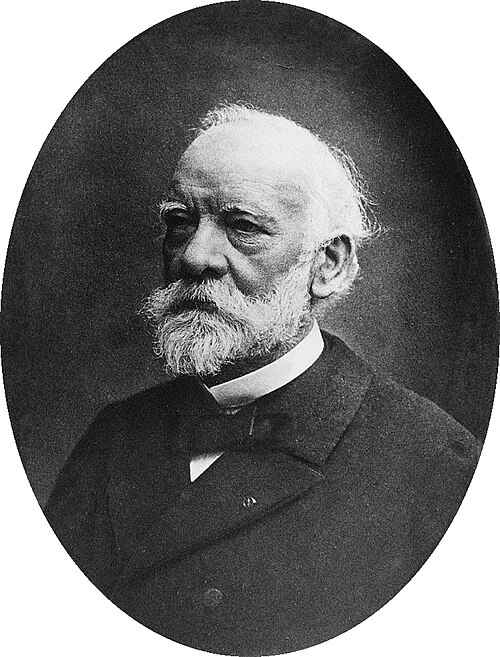
\includegraphics[width=\linewidth]{images/book3/friedel.jpg}
\end{minipage}\hspace{0.02\linewidth}%
\begin{minipage}[t]{0.18\linewidth}
\vspace{0pt}
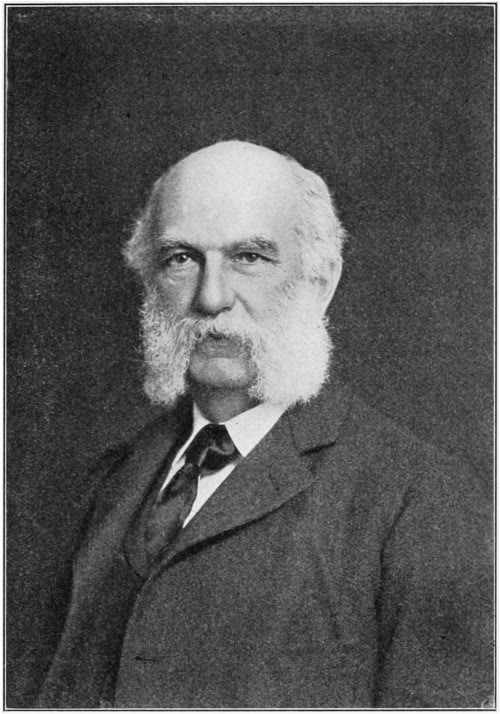
\includegraphics[width=\linewidth]{images/book3/crafts.jpg}
\end{minipage}\hfill
\begin{minipage}[t]{0.58\linewidth}
\vspace{0pt}
Pada tahun 1877 Charles Friedel dan James Mason Crafts, yang bekerja
bersama di Paris, menemukan bahwa aluminium klorida membuat haloalkana dan
asil klorida bereaksi dengan benzena. Reaksi-reaksi mereka menjadi cara baku
untuk memasang gugus karbon pada cincin \omterm{def:b2:huckel:aromatic}{aromatik}, dan katalisis asam Lewis
yang mereka temukan menjangkau jauh melampauinya. (Potret: Friedel, tahun
1890-an; Crafts, dari
\textit{Popular Science Monthly}, 1900; domain publik, Wikimedia Commons.)
\end{minipage}
\end{history}

\begin{safety}{\ghs[5mm]{GHS02}\,\ghs[5mm]{GHS05}\,\ghs[5mm]{GHS06}\,\ghs[5mm]{GHS08}}
Benzena bersifat karsinogenik dan diganti dengan toluena atau \omterm{def:b2:aromatic-substitution:arene}{arena} lain
bila memungkinkan. Asam nitrat dan asam sulfat pekat bersifat korosif dan
campuran penitrasi merupakan pengoksidasi kuat; campuran itu didinginkan dan
\omterm{def:b2:aromatic-substitution:arene}{arenanya} ditambahkan perlahan-lahan, karena nitrasi bersifat \omterm{def:b2:reaction-enthalpy:exothermic}{eksoterm}. Brom
sangat beracun dan korosif; aluminium klorida bereaksi hebat dengan air.
Nitroarena beracun.
% ledger: ghs:benzene, ghs:toluene, ghs:HNO3, ghs:H2SO4, ghs:Br2, ghs:AlCl3, ghs:nitrotoluene-4
\end{safety}

\section{Latihan}

\begin{exercise}[$\star$]\label{exo:b2:aromatic-substitution:1}
Tuliskan pembentukan ion nitronium dari asam nitrat dan asam sulfat.
\end{exercise}

\begin{exercise}[$\star$]\label{exo:b2:aromatic-substitution:2}
Tuliskan produk-produk utama brominasi (\ce{Br2}, \ce{FeBr3}) toluena dan
nitrobenzena.
\end{exercise}

\begin{exercise}[$\star$]\label{exo:b2:aromatic-substitution:3}
Golongkan sebagai pengaktif atau pendeaktif, orto/para atau meta: \ce{-CH3},
\ce{-OH}, \ce{-Cl}, \ce{-NO2}, \ce{-COCH3}, \ce{-NHCOCH3}.
\end{exercise}

\begin{exercise}[$\star$]\label{exo:b2:aromatic-substitution:4}
Tuliskan produk benzena dengan etanoil klorida dan aluminium klorida.
\end{exercise}

\begin{exercise}[$\star\star$]\label{exo:b2:aromatic-substitution:5}
Benzena dan 1-kloropropana dengan \ce{AlCl3} terutama menghasilkan
isopropilbenzena. Jelaskan, dan berikan jalur dua tahap menuju
propilbenzena.
\end{exercise}

\begin{exercise}[$\star\star$]\label{exo:b2:aromatic-substitution:6}
Fenol langsung menghilangkan warna air brom, tanpa katalis, dan
menghasilkan 2,4,6-tribromofenol. Jelaskan.
\end{exercise}

\begin{exercise}[$\star\star$]\label{exo:b2:aromatic-substitution:7}
Tuliskan sintesis 3-bromonitrobenzena dan 4-bromonitrobenzena dari benzena.
\end{exercise}

\begin{exercise}[$\star\star$]\label{exo:b2:aromatic-substitution:8}
Anilina sulit dinitrasi dengan baik (oksidasi, dan produk meta), tetapi
asetanilida terutama menghasilkan 4-nitroasetanilida. Jelaskan kedua fakta
itu.
\end{exercise}

\begin{exercise}[$\star\star$]\label{exo:b2:aromatic-substitution:9}
Tunjukkan bagaimana gugus asam sulfonat dapat dipakai untuk membuat 2-bromotoluena yang bebas dari isomer paranya.
\end{exercise}

\begin{exercise}[$\star\star\star$]\label{exo:b2:aromatic-substitution:10}
Di manakah 4-metilanisol (4-metoksitoluena) mengalami nitrasi? Jelaskan
dengan kedua gugus pengarahnya.
\end{exercise}

\begin{exercise}[$\star\star\star$]\label{exo:b2:aromatic-substitution:11}
2,4,6-Trinitrotoluena dibuat melalui tiga nitrasi berturut-turut terhadap
toluena, masing-masing dalam kondisi yang lebih keras. Jelaskan mengapa.
\end{exercise}

\begin{exercise}[$\star\star\star$]\label{exo:b2:aromatic-substitution:12}
Usulkan sintesis asam 4-nitrobenzoat dari toluena, dan sintesis asam 3-nitrobenzoat.
\end{exercise}

\section{Soal: Menitrasi Toluena}

\begin{problem}[{Soal akhir pekan --- ion nitronium dan mekanisme nitrasi,
posisi orto, meta, dan para toluena dibandingkan dengan rasio statistik,
pemisahan isomer-isomernya, dan neraca massa}]
\label{pb:b2:aromatic-substitution:1}
Data: titik leleh: 2-nitrotoluena \qty{-10}{\degreeCelsius}, 3-nitrotoluena
\qty{16}{\degreeCelsius}, 4-nitrotoluena \qty{52}{\degreeCelsius}. Data latihan
untuk satu percobaan: \qty{100}{g} toluena, \omterm{def:b2:continuous-reactors:conversion}{konversi} 90~\%, sebaran isomer
58~\% orto, 4~\% meta, 38~\% para. Massa molar (\unit{g/mol}): C 12.011,
H 1.008, N 14.007, O 15.999.
% ledger: mp:2-nitrotoluene, mp:3-nitrotoluene, mp:4-nitrotoluene, aw:C, aw:H, aw:N, aw:O

\medskip
\noindent\textbf{Bagian I --- Elektrofil dan mekanisme.}
\begin{enumerate}
  \item Tuliskan pembentukan ion nitronium.
  \item Gambarlah struktur Lewis-nya dan tentukan bentuknya.
  \item Tuliskan serangan \ce{NO2+} pada toluena di posisi para terhadap metil.
  \item Gambarlah ketiga struktur resonansi \omterm{def:b2:aromatic-substitution:seAr}{zat antara Wheland} para.
  \item Tahap manakah yang menentukan laju?
  \item Apa yang mengambil proton pada tahap kedua?
\end{enumerate}

\medskip
\noindent\textbf{Bagian II --- Ketiga posisi.}
\begin{enumerate}[resume]
  \item Berapa posisi orto, meta, dan para yang dimiliki toluena?
  \item Rasio berapakah yang akan dihasilkan oleh serangan acak?
  \item Gambarlah \omterm{def:b2:aromatic-substitution:seAr}{zat antara Wheland} meta dan jelaskan mengapa zat antara itu
        paling sedikit distabilkan.
  \item Bagaimana gugus metil menstabilkan zat antara orto dan para?
  \item Bandingkan rasio yang teramati dengan rasio statistik: posisi-posisi
        manakah yang disukai?
  \item Bandingkan rendemen per posisi pada orto (separuh persentase orto) dan
        pada para. Usulkan alasan perbedaannya.
  \item Apakah toluena dinitrasi lebih cepat atau lebih lambat daripada benzena?
\end{enumerate}

\medskip
\noindent\textbf{Bagian III --- Pemisahan.}
\begin{enumerate}[resume]
  \item Isomer manakah yang berwujud padat pada suhu kamar?
  \item Usulkan cara mengisolasinya dari campuran dengan pendinginan.
  \item Mengapa simetri mendukung titik leleh yang tinggi?
  \item Bagaimana isomer orto dan meta dapat dipisahkan sesudahnya?
  \item Mengapa isomer-isomer ini sulit dipisahkan dengan distilasi sederhana?
\end{enumerate}

\medskip
\noindent\textbf{Bagian IV --- Neraca massa.}
\begin{enumerate}[resume]
  \item Hitunglah massa molar toluena dan nitrotoluena.
  \item Hitunglah jumlah toluena dan nitrotoluena yang terbentuk.
  \item Hitunglah massa ketiga isomer.
  \item Reaksi lanjutan apakah yang harus dihindari dengan pendinginan dan
        dengan tidak memakai asam berlebih?
  \item Bagaimana asam 4-nitrobenzoat dapat dibuat dari isomer para?
  \item Nyatakan massa 4-nitrotoluena yang diperoleh dari \qty{100}{g} toluena
        dalam percobaan ini.
\end{enumerate}
\end{problem}
